\chapter{Implementierung}
\label{ch:Implementierung}

In diesem Kapitel wird erläutert, wie die Daten des Datensatzes gesammelt, zur weiteren Verarbeitung vorbereitet und schließlich analysiert werden.
Zur vollständigen Erarbeitung eines Datensatzes muss zuvor eine App erstellt werden, welche die zu sammelnden Daten der eSense Earpods empfängt und persistiert. 
Zudem soll die App den Ablauf einer Messung automatisch verwalten und danach einen einfachen Export der persitierten Daten ermöglichen.
Anschließend müssen die persistierten Daten aufbereitet werden, sodass sie klassifiziert werden können.

\section{App}
\label{ch:Implementierung:app}
Zur Erstellung des Datensatzes wurde eine App entwickelt.
Diese startet eine Messung, nachdem eine Verbindung zu den eSense-Earpods hergestellt wurde.
Jeder Messwert wird in der Datenbank abgespeichert.
In Abbildung \ref{implementation:app:erModel} ist das ER-Diagramm der Datenbank beschrieben.
Das Gerät wird bei der ersten Koppelung mit dem Namen und dessen Identifikator in der Tabelle {\glqq Device\grqq}abgespeichert.
Der Identifikator ist hierbei eine Repräsentation der MAC-Adresse, welche unter Swift nicht erreichbar ist.
Für jeden Messwert wird ein Eintrag in der Tabelle {\glqq EsenseData\grqq} abgelegt, sowie eine Referenz zu den \textit{x}, \textit{y} und \textit{z}-Achsenwerten der Gyroskop- und Beschleunigungsdaten, welche in der entsprechenden Tabelle abgelegt werden.
Zudem wird für jede Messung ein Zeitstempel (\texttt{timestamp}), eine Messungs-ID (\texttt{measurementID}), der aktuell auszuführende Task (\texttt{task}) und die Information, ob die LED des Smarphones an ist, oder nicht (\texttt{lightOn}) abgespeichert.

Die App ist in 3 Sektionen aufgeteilt, einer \textit{Chartansicht}, einer \textit{Messungsansicht}, sowie einer \textit{Einstellungsansicht}. 
(Abb. \ref{implementation:app:screenshots} Tabbar)
Im Weiteren wird nur die \textit{Messungsansicht} genauer erläutert, da die anderen Ansichten im Rahmen der Bachelorarbeit nicht relevant sind.

\begin{figure}[ht]
  \centering
  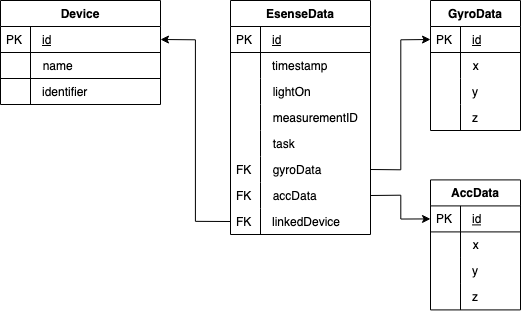
\includegraphics[width=0.7\textwidth]{implementation/app/Database_SleepEar}
  \caption{ER-Diagramm der App-Datenbank}
  \label{implementation:app:erModel}
\end{figure}

\newpage
\subsection{Messungsablauf}
\label{ch:Implementierung:app:measurement_procedure}
Mit der Messungsansicht soll eine komplette Messung durchgeführt werden.
Der \textit{MeasurementFlow} wird gestartet und die erste \textit{View} (Abb. \ref{implementation:app:screenshots:connect_bluetooth}) wird geöffnet.
Nach der erfolgreichen Verbindung mit den eSense-Earpods erfolgt eine Weiterleitung zur nächsten \textit{View} (Abb. \ref{implementation:app:screenshots:user_studies_information}) zum Ausfüllen der Nutzerinformationen. 
Mit dem Betätigen des Buttons: {\glqq Start Measurement\grqq} bestätigt man die Eingabe der Daten und die Messung beginnt.
Automatisch beginnt der erste Timer (Abb. \ref{implementation:app:screenshots:measurement_started}).
Der Timer zeigt den aktuellen, sowie den nächsten \textit{Task} an, sowie die Restzeit des aktuellen Tasks.
Der genaue Ablauf der einzelnen Timer ist in Abbildung \ref{fig_study_flow} detailliert beschrieben.
Nach dem Ablauf des letzten Timers wird eine View geöffnet, welche die Möglichkeit zum Teilen der aktuellen Messung bietet (Abb. \ref{implementation:app:screenshots:sampling_stopped}, \ref{implementation:app:screenshots:share}).
Zudem kann die Datenbank vollständig geleert werden.
Während dieses Ablaufs wird ein Objekt erstellt, welches die Messung verwaltet.

\subsection{Messung}
\label{ch:Implementierung:app:measurement}
Eine Messung wird im Code in einem \textit{Measurement} Objekt persistiert.
Durch ein Observer-Pattern wird der \textit{MeasurementFlow} über jegliche Änderung informiert und kann entsprechende Handlungen durchführen.
Durch die Funktionen \texttt{startMeasurement} und \texttt{stopMeasurement} kann eine Messung gestartet, beziehungsweise gestoppt werden.
Mit der Funktion \texttt{startMeasurement} wird das IMU-Sampling per BLE, sowie die Audioaufnahme gestartet. 
Ebenso wird der erste Timer gestartet und ein doppeltes Lichtsignal wird gesendet. 
Durch die Funktion \texttt{stopMeasurement} werden die Datenströme gestoppt, ebenfalls ein doppeltes Lichtsignal gesendet und der Timer wird beendet.
Der nächste Task wird gestartet, wenn der Timer abgelaufen ist. Der Timer startet mit der Länge des nächsten Tasks.
Sofern der nächste Task {\glqq Hold\_breath\grqq} ist, also die Person im folgenden Task die Luft anhält, wird dem Teilnehmer kurz vor Ablauf mitgeteilt, wann der nächste Task startet.
Mit der Instruktion \glqq Bitte die Luft anhalten in 3, 2, 1\grqq \ weiß der Teilnehmer, wann er die Luft anhalten soll.
Durch die Anweisung \glqq Stopp\grqq \ wird dem Nutzer das Ende des Tasks mitgeteilt. 
Die Instruktionen liegen als Audiodatei vor und werden jeweils vor dem jeweiligen Task abgespielt und mittels Bluetooth über die Lautsprecher der eSense-Earpods ausgegeben.

\newpage
\section{Anbindung an die Auswertungspipeline}
\label{ch:Implementierung:way_to_pipeline}
\begin{wrapfigure}{r}{0.3\textwidth}
  \centering
  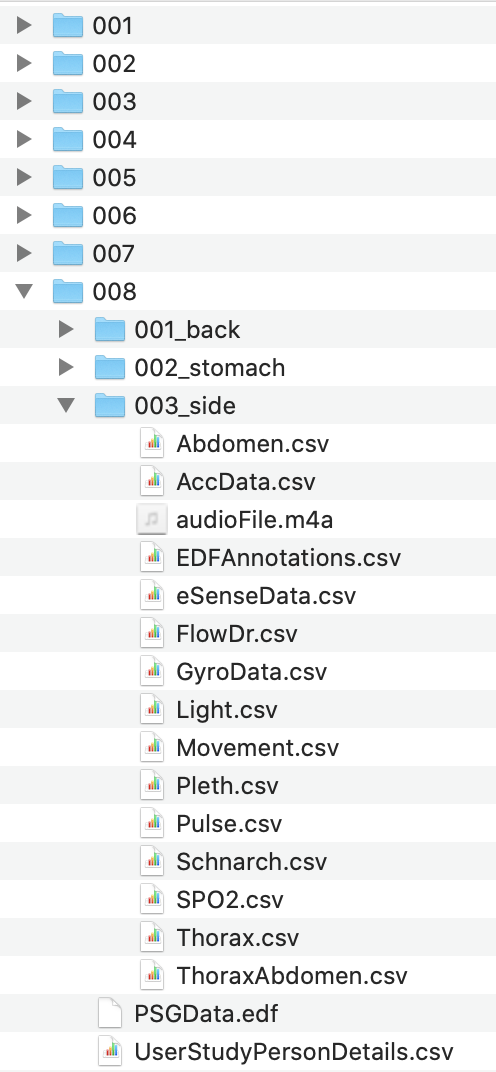
\includegraphics[width=0.25\textwidth]{data_analyzation/folder_structure}
  \caption{Ornderstruktur des Datensatzes}
  \label{implementation:folder_structure}
\end{wrapfigure}
Die App liefert beim Export die Daten der eSense-Earpods, was die IMU-Daten, sowie die Nutzerinformationen und die Mikrofonaufnahme beinhaltet.
Zum aktuellen Stand liegen somit die Daten der eSense-Earpods und die des PSG-Systems vor. 
Zu Beginn müssen die PSG-Daten, welche als eine Messung für alle 3 Positionen pro Studienteilnehmer persistiert wurde, in 3 einzelne Messungen aufgeteilt werden.
Die Daten des PSG-Systems liegen als \textit{edf}-Datei vor. 
Diese können mittels Python und der Library \texttt{edfrd} ausgelesen werden.
Jedoch sind die Einträge des jeweiligen Signals ohne einen Zeitwert abgespeichert. 
Es muss nun aufgrund der Abtastrate in $\si{\hertz}$ die Zeit manuell berechnet werden. 
Mittels der Funktion \texttt{find\_peaks} aus \texttt{scipy.peak}\ können die Peaks des Lichtsensors am PSG-System ermittelt werden (siehe Abb. \ref{implementation:synchronisation:light_peaks_detection}).
Da eine Messung mit 2 Lichtblitzen beginnt und endet, kann nun der Start- und Endzeitpunkt einer Position ermittelt werden. 
Die einzelnen Positionen können sodurch voneinander unterschieden werden. 
Daraufhin können die 11 verfügbaren Signale einzeln ausgelesen werden.
Pro Position wird nun jedes der Signale als \textit{csv}-Datei im jeweiligen Ordner abgelegt.
Die Daten der eSense-Earpods liegen getrennt in \textit{AccData\_\$ID\$.csv} und \textit{GyroData\_\$ID\$.csv} vor. 
Diese werden ausgelesen und zu der Datei \textit{eSenseData.csv} zusammengeführt.
Die Ordnerstruktur kann der Abbildung \ref{implementation:folder_structure} entnommen werden und ist nun vollständig.

\begin{figure}[ht]
  \centering
  \begin{subfigure}{.25\textwidth}
    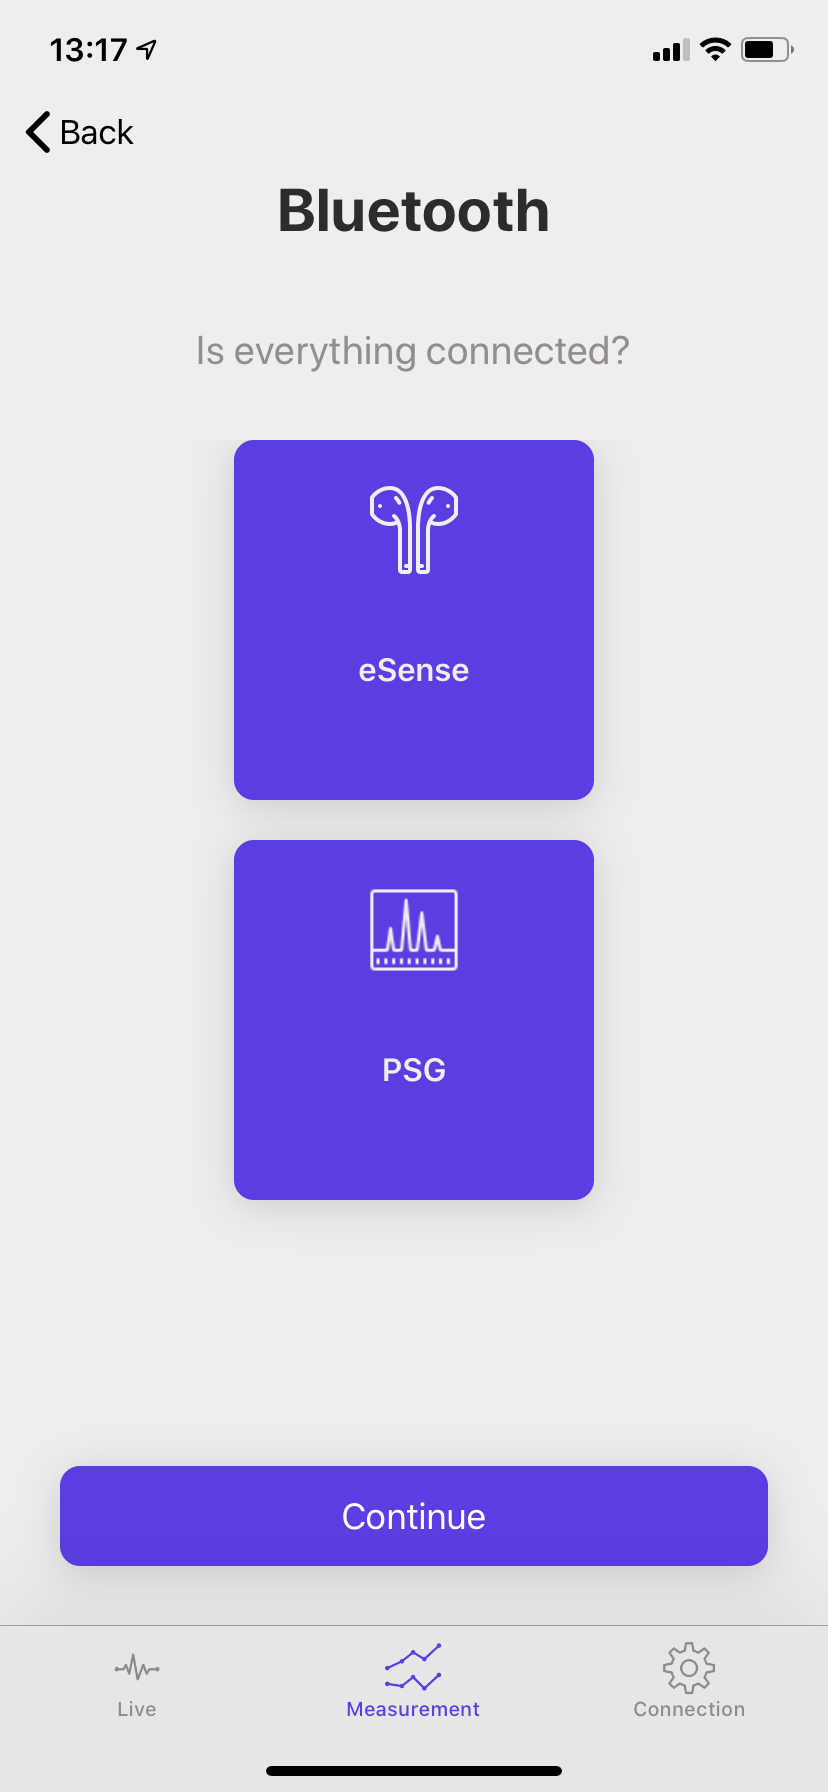
\includegraphics[width=1\textwidth]{app/connect}
    \caption{Verbinden der eSense-Earpods}
    \label{implementation:app:screenshots:connect_bluetooth}
  \end{subfigure}
  \begin{subfigure}{.25\textwidth}
    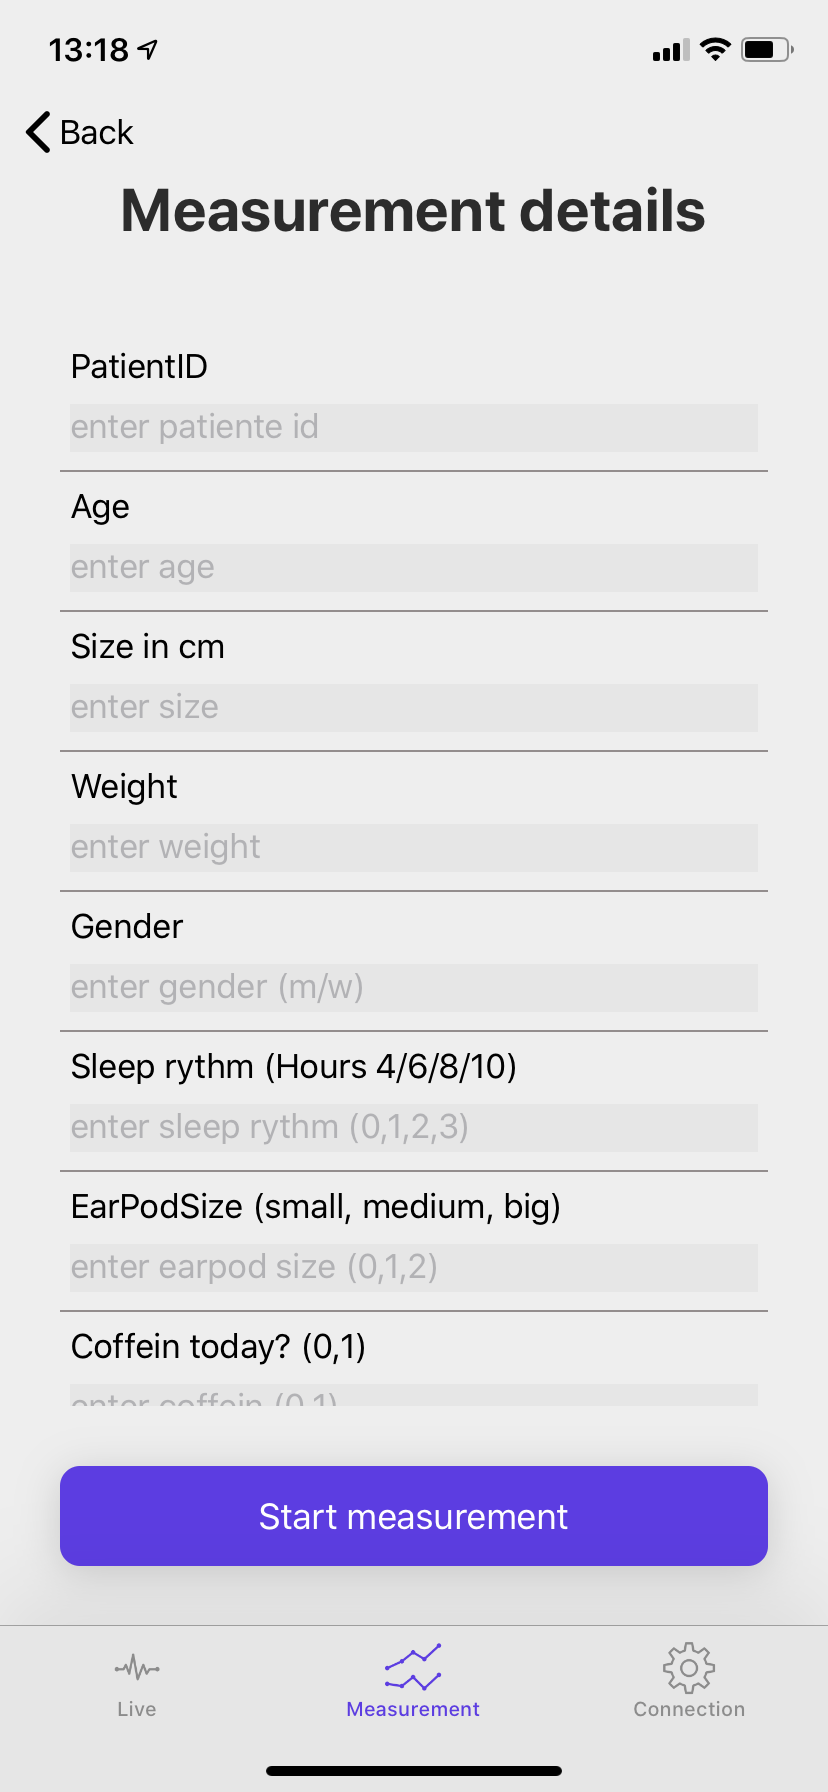
\includegraphics[width=1\textwidth]{app/measurement_details}
    \caption{Eingabe der Nutzerinformationen}
    \label{implementation:app:screenshots:user_studies_information}
  \end{subfigure}
  \begin{subfigure}{.25\textwidth}
    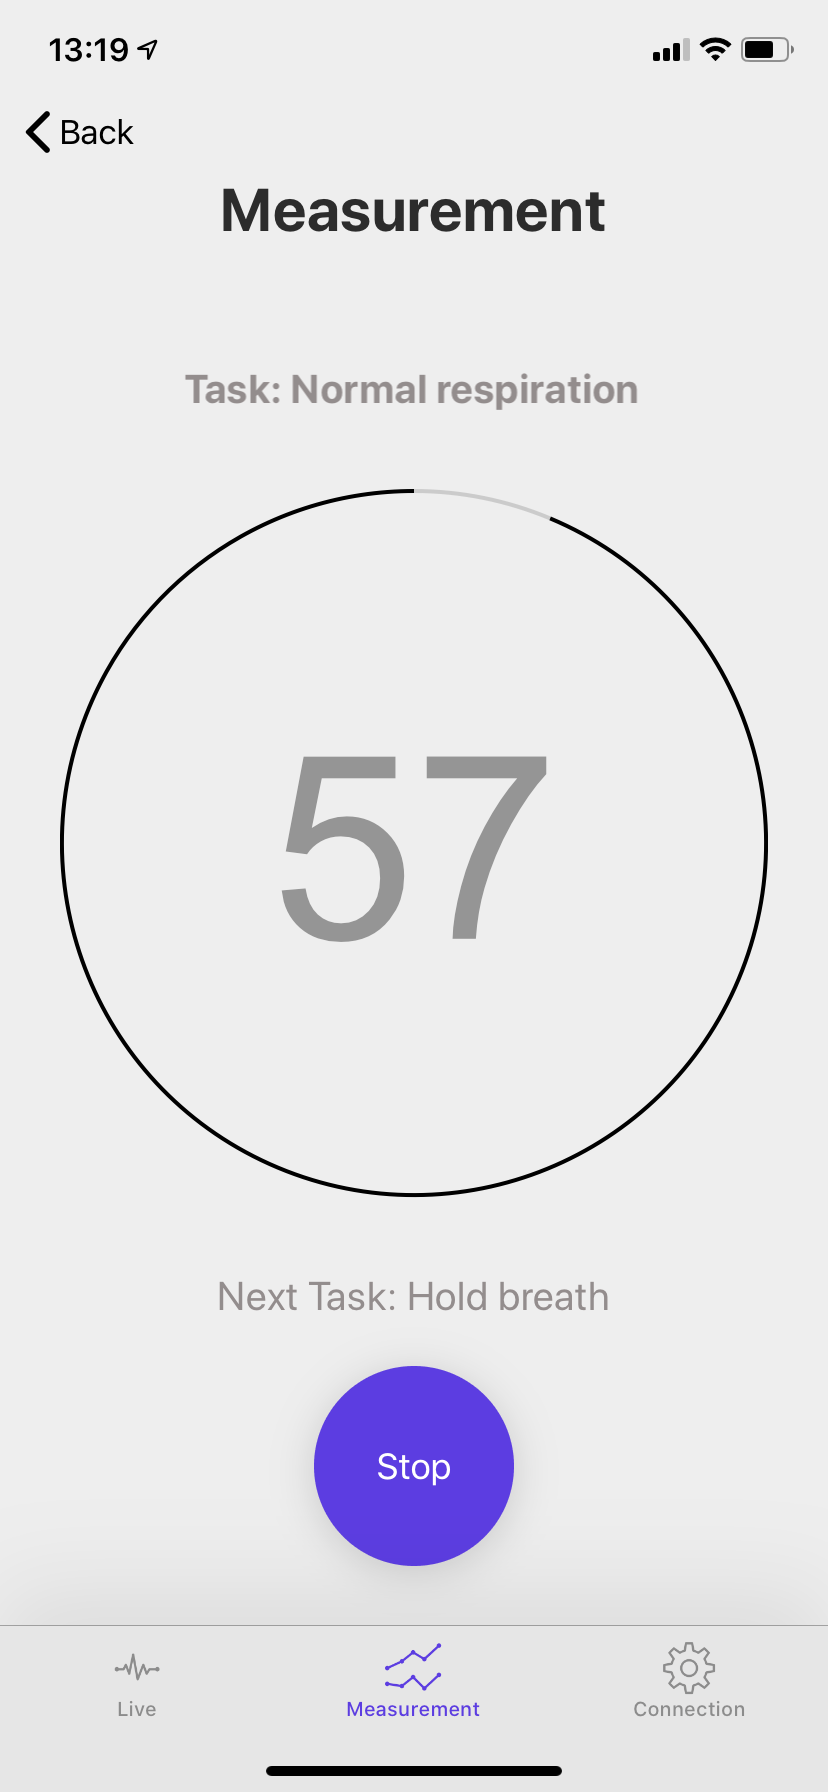
\includegraphics[width=1\textwidth]{app/measurement_timer_02}
    \caption{Messung, aktueller und nächster Task}
    \label{implementation:app:screenshots:measurement_started}
  \end{subfigure}
  \begin{subfigure}{.25\textwidth}
    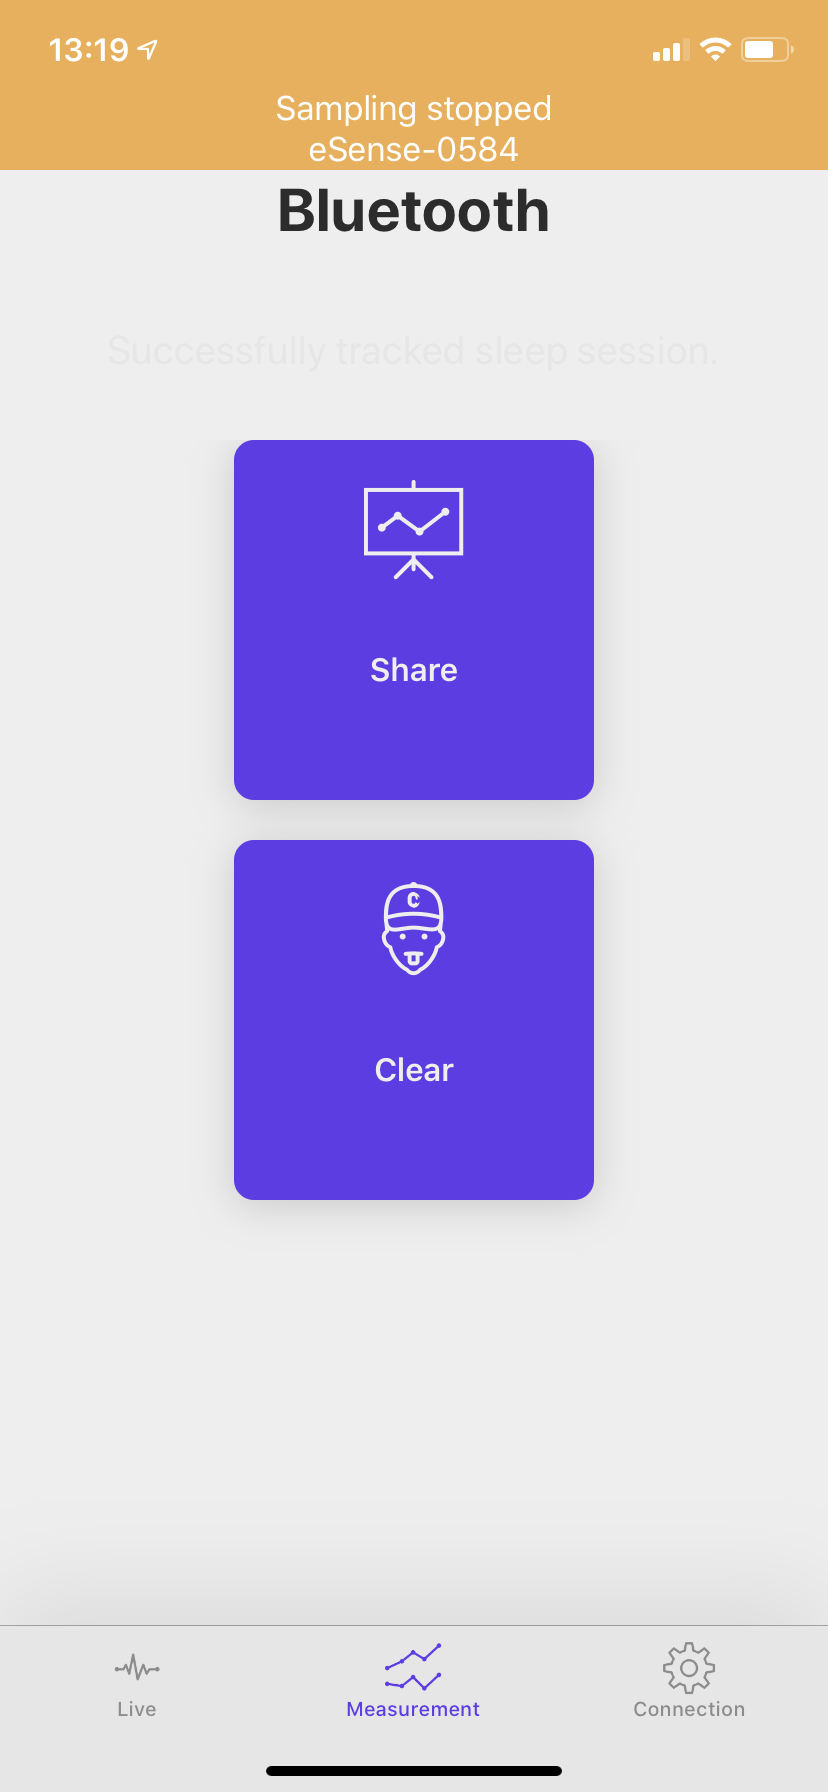
\includegraphics[width=1\textwidth]{app/measurement_finished}
    \caption{Messung beendet}
    \label{implementation:app:screenshots:sampling_stopped}
  \end{subfigure}
  \begin{subfigure}{.25\textwidth}
    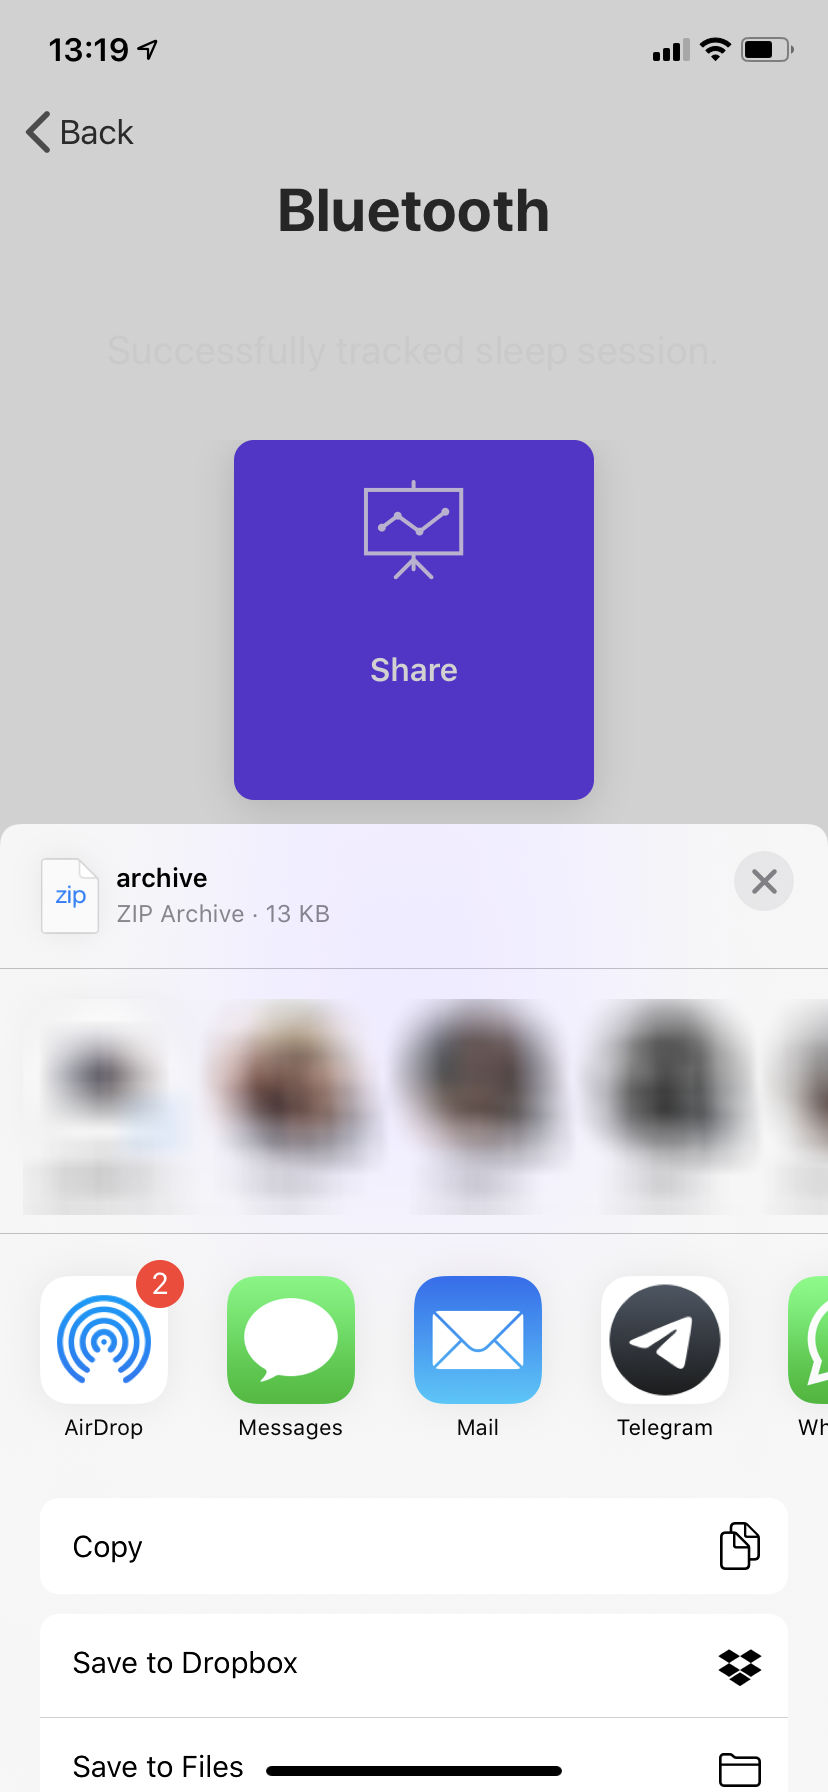
\includegraphics[width=1\textwidth]{app/measurement_share}
    \caption{Messung teilen}
    \label{implementation:app:screenshots:share}
  \end{subfigure}
  \caption{Verlauf einer Messung mit der App: Zu Beginn wird eine Verbindung mit den eSense-Earpods hergestellt, anschließend werden die Nutzerinformationen des Probanden abgefragt. Mit dem Klick auf \textit{Start Measurement} wird eine Messung gestartet. Der erste Timer läuft ab und über die Lautsprecher werden alle Information an den Probanden weitergegeben. Nach Ablauf des Timers beginnt der nächste Timer. Sobald der letzte Timer abgelaufen ist, kann die Messung geteilt werden. Zudem kann die Datenbank gelöscht werden und die nächste Messung kann beginnen. Der Ablauf einer Messung ist in Abbildung \ref{fig_study_flow} nachzusehen.}
  \label{implementation:app:screenshots}
\end{figure}

\subsection{Synchronisation der Daten}
\label{ch:Implementierung:data_sync}
Da es nicht garantiert ist, dass der Timer des PSG-Systems zuverlässig arbeitet, wird jeder Peak des Lichtsensors mit dem Lichtsignal der Smartphone-Daten verglichen.
Der Abstand jedes einzelnen Peaks wird nun ermittelt, ebenso wie die durchschnittliche Distanz der Peaks.
In der Abbildung \ref{implementation:synchronisation:before_light_peak} ist der Vergleich eines Lichtblitzes von Smartphone (blau) und dem PSG-System (orange) im zeitlichen Verlauf dargestellt (\texttt{time}).
Da die Verschiebung des Timers des PSG-Systems während einer 7-minütigen Messung im Mittel bei $0.3\si{\s}$ lag, wurde der Timer des PSG-Systems um die durchschnittliche Distanz der Peaks verschoben.
Dies ist ausreichend, da die PSG-Daten in der Bachelorarbeit lediglich dem visuellen Vergleich dienen und in der Klassifikation nicht mit betrachtet werden. 
Die zeitliche Verschiebung wird nun in jede \textit{csv}-Datei mit der Spalte \texttt{new\_time} eingearbeitet.
In Abbildung \ref{implementation:synchronisation:after_light_peak} ist klar zu erkennen, dass der neue Zeitwert (\texttt{new\_time}) des PSG-Signals (orange) direkt über dem Zeitwert des Smartphonesignals (blau) liegt, was an den Lichtpeaks zu erkennen ist.
Nun ist garantiert, dass die Lichtsignale von PSG-System und dem Smartphone annähernd synchron sind. Die Daten sind nun bereit zur Analyse.

\begin{figure}[ht]
  \centering
  \begin{subfigure}{0.66\textwidth}
    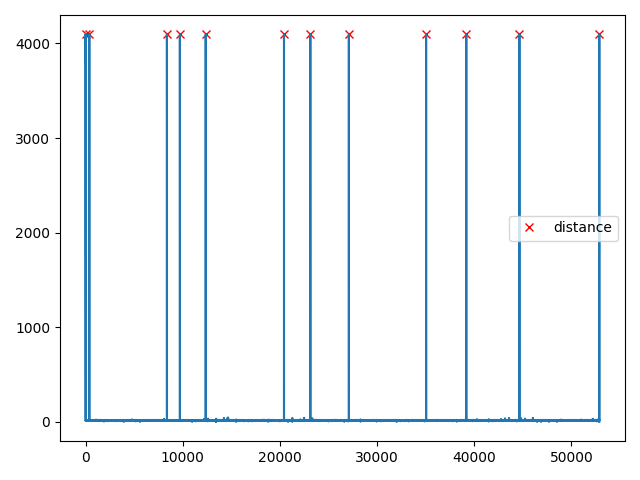
\includegraphics[width=1\textwidth]{data_analyzation/light_peak_detection_psg_data}
    \caption{Peaks des Lichtsignals vom PSG-Gerät. Somit können die PSG-Daten und die Daten, gesammelt von den eSense Earpods zeitlich synchronisiert werden. Der Ablauf der Lichtpeaks ist identisch zum Ablauf der Nutzerstudie (siehe Abb. \ref{fig_study_flow}). Die y-Achse zeigt den Lichtausschlag des Sensors, die x-Achse den Zeitwert.}
  \end{subfigure}
  \begin{subfigure}{.49\textwidth}
    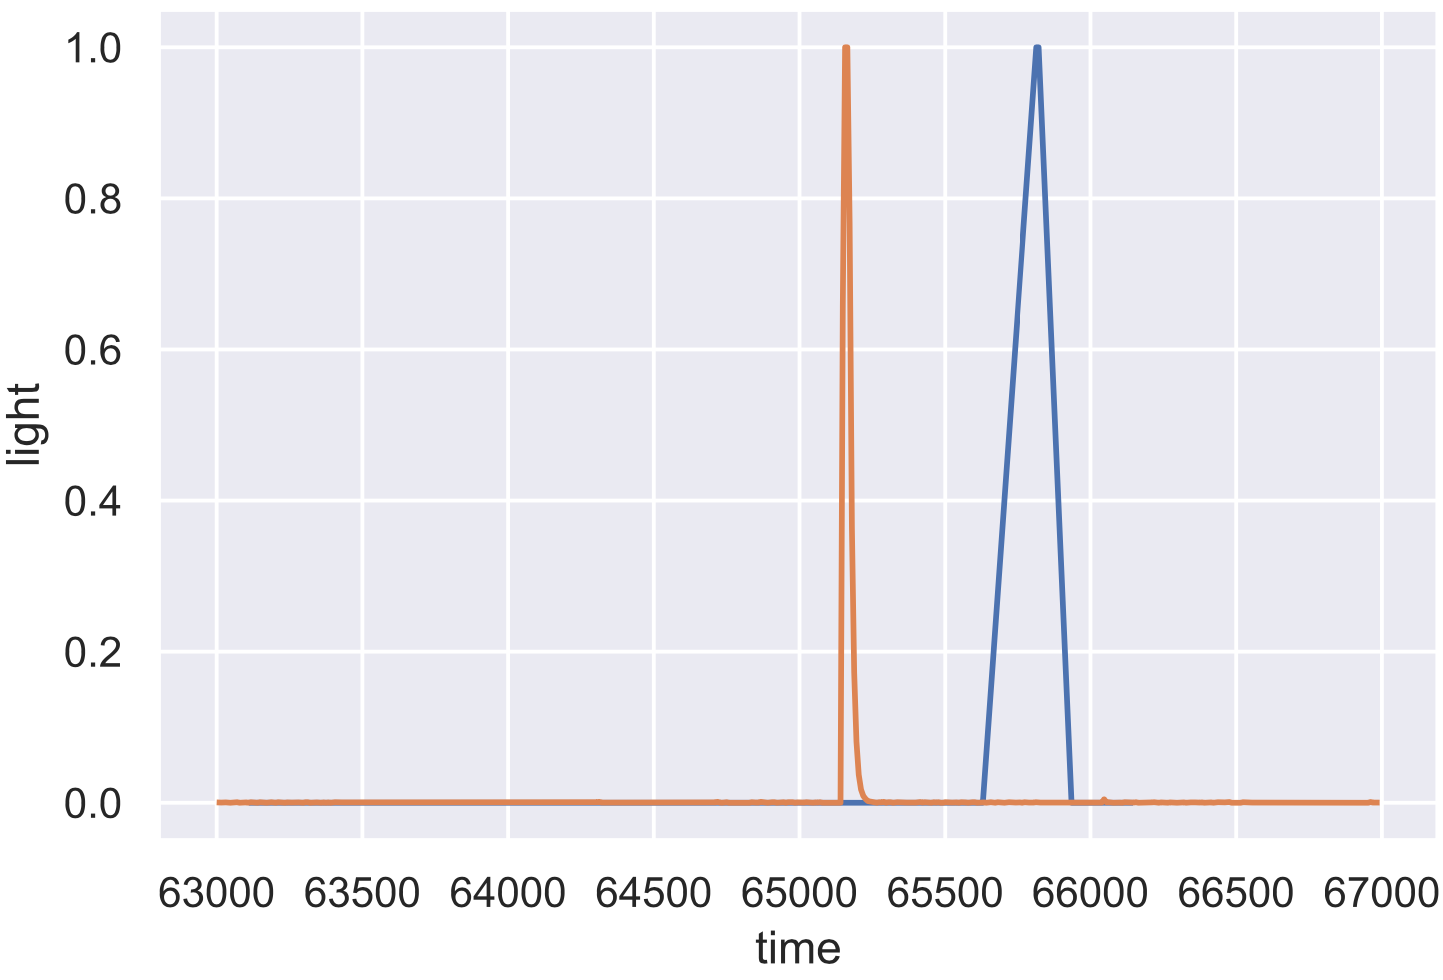
\includegraphics[width=1\textwidth]{data_analyzation/light_peak_detail_before.png}
    \caption{Zeitlicher Lichtpeakvergleich vor der Synchronisation. Das Lichtsignal des PSG-Geräts (orange) ist weniger als 1s vom Signal der eSense Earpods (blau) entfernt. Der Zeitwert ist in $\si{\ms}$ angegeben. Die Lichtsignale wurden skaliert, um diese vergleichen zu können. }
    \label{implementation:synchronisation:before_light_peak}
  \end{subfigure}
  \begin{subfigure}{.49\textwidth}
    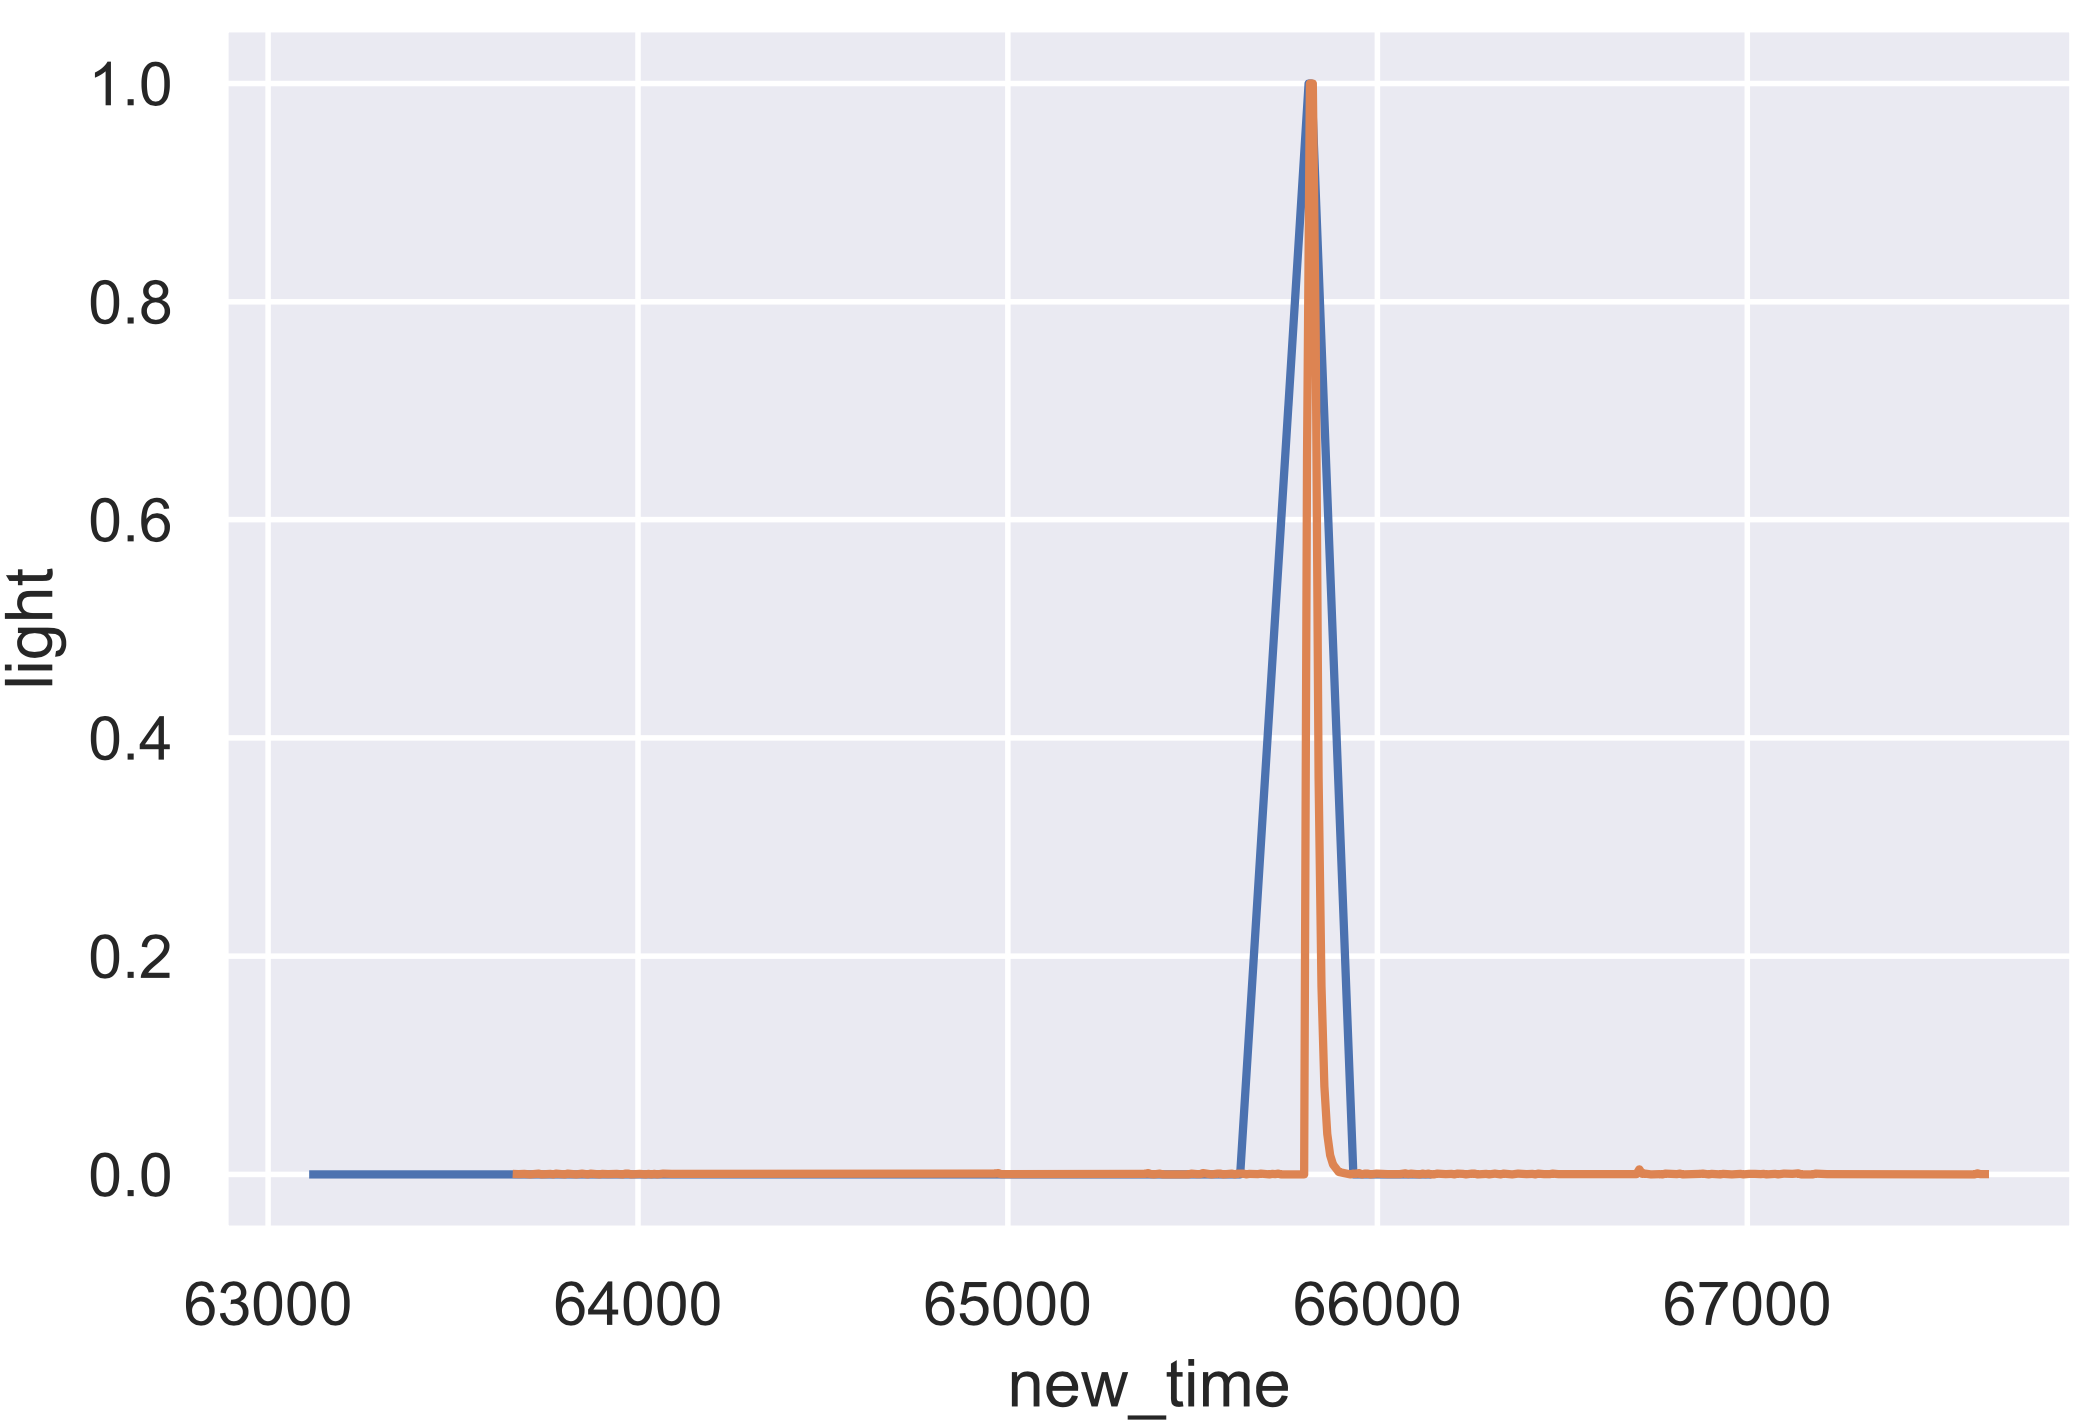
\includegraphics[width=1\textwidth]{data_analyzation/light_peak_detail_after.png}
    \caption{Zeitlicher Lichtpeakvergleich nach der Synchronisation. Das Lichtsignal des PSG-Systems (orange) ist nun zeitlich sehr nahe über den Lichtpeaks der eSense Earpods (blau). Der neue Zeitwert ist in der Spalte \texttt{new\_time} jeder Datei zu entnehmen. Der Zeitwert ist in $\si{\ms}$ angegeben.}
    \label{implementation:synchronisation:after_light_peak}
  \end{subfigure}
  \label{implementation:synchronisation}
\end{figure}

\newpage
\section{Verarbeitungspipeline zur Klassifikation}
\label{ch:Implementierung:classification_pipeline}
Zur Klassifizierung der Daten müssen nun Features berechnet werden. 
Diese werden jedoch nicht auf das ganze Zeitintervall einer Messung berechnet, sondern aufgeteilt.
Eine Messung wird nun in Fenster der Größe von 5 bzw. 10 Sekunden aufgeteilt, wobei jedes Fenster um eine Sekunde verschoben wird. 
Somit überlappen sich zwei aneinander liegende Fenster immer um 4 bzw. 9 Sekunden. 
Die Trennung der Fenster wurde anhand des Zeitwertes jedes Messergebnisses entschieden, da die Messergebnisse der eSense Earpods beim Senden per BLE an das Smartphone keine Uhrzeit beinhalteten.
Dadurch liegt kein genauer Abstand der einzelnen Messdaten von $50\si{\hertz}$ vor. 
Anschließend wurden mittels des Moduls \texttt{tsfresh} Features für jedes Fenster einzeln berechnet und es entstand eine Datei \textit{df\$patient\_id\$\_\$position\_id\$\_feature.csv}, welche alle Features der einzelnen Fenster beinhaltet.

Da nun die Features für eine Fenstergröße von $5\si{\s}$ und $10\si{\s}$ mit der Verschiebung von $1\si{\s}$ pro Fenster vorliegen, kann mit der Klassifikation begonnen werden.